\documentclass[a4paper, 11pt]{scrartcl}

\usepackage[utf8]{inputenc} % gestion des accents (source)
\usepackage[T1]{fontenc} % gestion des accents (PDF)
%\usepackage[francais]{babel} % gestion du français
\usepackage[english]{babel} % gestion du français
\usepackage{textcomp} % caractères additionnels
\usepackage{xcolor}
\usepackage{caption}
\usepackage{subcaption}
\usepackage{lmodern} % police de caractères

\newcommand{\jump}{\vspace{0.3cm}}

\usepackage[bookmarks=true]{hyperref} % liens hypertexte
\hypersetup{
  colorlinks,
  citecolor=violet,
  linkcolor=black,
  urlcolor=blue}
%\usepackage{pstricks} % encadrage

\usepackage{graphicx}
\usepackage{caption}
\usepackage{amsmath, amsfonts, amssymb}
%\usepackage{listings}
%\usepackage[fancysections]{polytechnique}
\usepackage{fancyhdr}
\usepackage{eso-pic,xcolor,graphicx}
\definecolor{light-gray}{gray}{0.7}

\pagestyle{fancy}
%\usepackage[top=1in, bottom=1.25in, left=1in, right=1in]{geometry}

%\lhead{Convex Neural Networks} 
%\chead{\today}
%\rhead{Eloïse \textsc{Berthier}}

\newtheorem{theorem}{Theorem}[section]
\newtheorem{definition}{Definition}[section]
\newtheorem{proposition}{Proposition}[section]
\newtheorem{corollary}{Corollary}[theorem]
\newtheorem{lemma}[theorem]{Lemma}

\title{On Convex Neural Networks}
\author{Eloïse Berthier}
\date{\today}
\subtitle{Mathematical Foundations of Data Science}


\begin{document}

\setcounter{secnumdepth}{3}
\setlength{\parindent}{0cm}

\maketitle
%\fontfamily{lmss}\selectfont

\everymath{\displaystyle}

\abstract{
\emph{1/2 page: What problem(s) is studied ? 
Why is it relevant ? 
What solution(s) is proposed ? 
Which contributions (theory, numerics, etc) ? 
}}

\newpage

\section{Introduction}

While the use of neural networks has dramatically increased the performance of some recognition systems, there still lacks a clear mathematical understanding of this success. One of the key issues is that optimizing neural networks is a non-convex problem, hence training algorithms may not return a global minimum.

Yet in practice, training large neural networks often results in satisfying solutions, which are empirically considered \textit{not too far} from a global minimum. Thus it suggests that there may be some implicit assumptions on the data or on the model that are usually verified and could explain this regularity, somehow making the problem \textit{more convex} than at first sight.\\

There have been several attempts to study this phenomenon, heading in different directions. Here are some examples.

Some rely on convex relaxations of the original optimization problem. \cite{zhang2016convexified} define a convex relaxation for training convolutional neural networks. They show that in the case of a two-layer CNN, the generalization error of the solution to the convex relaxed problem converges to that of the best possible two-layer CNN.

In \cite{haeffele2017global} are studied conditions under which the optimization landscape for the non-convex optimization problem is such that all critical points are either global minimizers or saddle points. \cite{visualloss} provide a tool to visualize the loss surface along random directions near the optimal parameters.

There is also a series of some very recent contributions on the problem: \cite{du2018agradient}, \cite{du2018bgradient} and \cite{zou2018stochastic}. They rely on the analysis of the dynamics of the prediction space rather than of the parameter space, the former being governed by the spectral property of a Gram matrix. If the data are \textit{not degenerate}, this Gram matrix’s least eigenvalue is lower bounded, and randomly initialized gradient descent linearly converges to a global optimum.

In the infinite-width limit, \cite{jacot2018neural} relate the evolution of a neural network function to a kernel that they call the \textit{neural tangent kernel}. Convergence to a global minimum can then be related to the positive-definiteness of the limiting kernel, and which is the case when the data are on a sphere.

However, \cite{chizat:hal-01945578} notice that part of these results may be explained by a specific \textit{lazy} training setting which does not reflect practical deep learning applications. \\

In this report, we concentrate on another approach called \textit{convex neural networks}. The core idea was introduced by \cite{bengio2006convex} and focuses on one hidden-layer neural networks. Instead of optimizing the weights of a network with a fixed number of hidden units, we could consider the equivalent problem of optimizing on the set of all the possible hidden unit functions. The training problem is convex with respect to the parameters of the model (which are now only the ouput weights).

Of course, while this approach solves the non-convexity issue, it introduces some other difficulties. These are extensively studied in \cite{bach2017breaking}, on which we will mainly focus in this report. A complete analysis of the generalization performance of convex neural networks is derived, in particular showing that high-dimensional non-linear variable selection may be achieved, without any strong assumption regarding the data. Yet this approach requires to solve a convex problem in infinite dimension and is only possible if the non-convex subproblem of adding a new hidden unit can be solved efficiently. Finding a polynomial-time algorithm solving this subproblem induced by the conditional gradient method is still an open question.

\cite{chizat2018global} focus on solving the same convex problem, but avoid the potentially NP-hard problem of optimizing with conditional gradient. Instead, they discretize the unknown measure as a mixture of particles. This approach is inspired by optimal transport and brings strong asymptotical global optimality guarantees for gradient flow optimization. It also provides simple numerical experiments.\\

Looking at all these different approaches, we may notice some recurrent patterns in the assumptions that are commonly made:

\begin{itemize}
\item \textit{one hidden-layer models}: most of the articles focus on simple neural network models, that already include a wide variety of classical supervised learning configurations, but do not directly cover deep neural networks.
\item \textit{over parametrization}: all the good generalization properties are derived in the case of an over parametrized model, yet the key question is \textit{how much} over parametrization is needed.
\item \textit{positive homogeneity}: most of the results are achieved in the case of positively homogeneous activation functions. It could explain the experimental advantage of using ReLU functions over others in deep learning.
\item \textit{proper initialization}: several articles rely on the conservation of an initial regularity through the optimizing process, for instance using gradient flows, and so emphasize the role of the initialization.
\end{itemize}

\section{Towards a Convex Problem}

\subsection{General layout}

We consider single hidden-layer neural networks. It defines a class of prediction functions on $\mathbb{R}^d$ parametrized as: $f_{\eta, b, v}(x) =\sum_{j=1}^k \eta_j \sigma(v_j^\top x + b_j)$, where $\sigma$ is a fixed activation function, $k$ is the number of hidden units, $v_j$ and $b_j$ are the weight and bias of layer $j$ and $(\eta_j)_{j=1,...,k}$ the weights of the output layer. We can eliminate the $b_j$ by integrating it into $v_j$ and adding a one on top of $x$.\\

We will mainly consider a fixed non-decreasing and positively homogeneous  activation function of some integer degree, i.e. $\sigma(u) = (u)^\alpha_+$, for some $\alpha \in \mathbb{N}$ (it includes ReLU and hard-thresolding functions). We will also later consider sigmoid activation functions in the numerical experiments.

\subsection{From non-convexity to convexity}

For a fixed value of $k$, training a neural network is an empirical risk minimization problem: $\min_{\eta, v} \frac{1}{n} \sum_{i=1}^n \ell(f_{\eta, v}(x_i), y_i) + \Omega(\eta, v)$, where $\ell$ is a smooth convex loss function (convex in its first argument) and $\Omega$ a convex regularization function, and $(x_i, y_i)$ the observations in $\mathcal{X} \times \mathbb{R}$. This is not a convex problem because of the non-convexity of the prediction function.\\

Now consider the set $\mathcal{F}_\mathcal{V}$ of all the possible hidden unit functions $\varphi_v : \mathcal{X} \rightarrow \mathbb{R}$, with $\mathcal{X}$ any measurable space. We will call it the set of basis functions. It is parametrized by the compact topological space $\mathcal{V}$ of all possible hidden unit weight vectors. We assume that for all $x \in \mathcal{X}$, the functions $v \mapsto \varphi_v(x)$ are continuous. To represent any affine function, $\mathcal{V}$ has dimension $d + 1$ for inputs in $\mathcal{X}$ of dimension $d$.

Let $\mathcal{W}$ be the Hilbert space of functions from $\mathcal{F}_\mathcal{V}$ to $\mathbb{R}$, with $\cdot$ an inner product. For any $x \in \mathcal{X}$, we define $h(x)$ as the function that maps any $\varphi_v \in \mathcal{F}_\mathcal{V}$ to $\varphi_v(x)$. $h(x)$ is an element of $\mathcal{W}$. $h(x)$ can be seen as the vector of activations of the hidden units when we observe $x$ as input. An element $\eta$ of $\mathcal{W}$ can also be understood as the output weights vector in a neural network. We extend the definition of $\Omega$ to be a convex regularization functional from $\mathcal{W}$ to $\mathbb{R}$.  \\

We can define the following problem:
\begin{equation}
\min_{\eta \in \mathcal{W}} \mathcal{C}(\eta) = \frac{1}{n} \sum_{i=1}^n \ell(\eta \cdot h(x_i), y_i) + \Omega(\eta)
\end{equation}

\begin{lemma}
Problem (1) is a convex minimization problem.
\end{lemma}
The proof is straightforward: any Hilbert space $\mathcal{W}$ is convex, $ \ell(\eta \cdot \varphi(x_i), y_i)$ is convex in $\eta$ and by additivity the objective function also is.\\

This problem formulation is from \cite{bengio2006convex}. It is a bit hard to handle as it introduces many notations that are not all explicit. Still it provides an intuitive idea of the problem we want to define: considering all the possible hidden units we could pick, how to combine them to make a good prediction, that is, how to choose the output weight $\eta$ to minimize $\mathcal{C}$. 

In this problem the penalization term is crucial. Unlike the initial optimization problem where the number of hidden units was fixed, it is now part of the optimization problem. Without any regularization, the solution could have an arbitrary large number (possibly infinite) of non-zero variables $\eta_j$. We will later see that a proper regularization can ensure a finite number of selected units, and so a finite model.

$\mathcal{W}$ is the space of the output weights, and since it has infinite dimension, it is handled as a space of functions. What makes it a bit entangled is that eventually $\mathcal{W}$ is defined as a space of functions (output layer) of functions (hidden layer) of $x\in \mathcal{X}$, but it can also be seen as a simple vector (in potentially infinite dimension). The vector of activations of the hidden layer for a fixed input $x$ is also an element of $\mathcal{W}$ because it has the same shape as $\eta$. Notice that due to these notations, this formulation could hardly be generalized to a greater number of layers.\\

For the rest of this report, we will focus on the more general problem formulation in \cite{bach2017breaking}, which defines two spaces $\mathcal{F}_1$ and $\mathcal{F}_2$, for which we do not explicitely define an output Hilbert space $\mathcal{W}$. In fact, we do not actually manipulate the parameters of the neural network, but we will rather directly optimize on end-to-end neural network fonctions $f \in \mathcal{F}_1$ or $\mathcal{F}_2$. To take the penalty into account, we will have to define a notion of norm on these spaces, and discrete Radon measures will now play the role of the output weights $\eta$.

\subsection{Variation norm}

To properly define $\mathcal{F}_1$, we have to introduce Radon measures.

\begin{definition}
Real-valued Radon measures are continuous linear forms on the space of continuous functions from $\mathcal{V}$ to $\mathbb{R}$, equipped with the uniform norm.
\end{definition}

The total variation norm $|\mu|(\mathcal{V})$ of a Radon measure $\mu$  is equal to the supremum of $\int_\mathcal{V} g(v)\textnormal{d}\mu(v)$, over all continuous functions $g$ with values in $[-1, 1]$. When $\mu$ has a density with respect to a fixed probability measure $\tau$, ${d}\mu(v) = p(v) {d}\tau(v)$, then this is the $L^1$ norm of this density: $$|\mu|(\mathcal{V}) = \int_\mathcal{V} |p(v)| \textnormal{d}\tau(v)$$
When the measure is discrete, that is $\mu = \sum_{j=1}^k \eta_j \delta_{v_j}$ the total variation of $\mu$ is the $\ell^1$-norm of $\eta$:
$$|\mu|(\mathcal{V}) = \sum_{j=1}^k |\eta_j|  $$

\begin{definition}
$\mathcal{F}_1$ is the space of functions $f$ that can be written as
$f(x)= \int_\mathcal{V} \varphi_v(x)\textnormal{d}\mu(v)$,
where $\mu$ is a signed Radon measure on $\mathcal{V}$ with finite total variation.
\end{definition}

\begin{definition}
The variation norm of $f \in \mathcal{F}_1$ with respect to $\mathcal{V}$ is the infimum of $|\mu|(\mathcal{V})$ over all decompositions of $f$ as $f= \int_\mathcal{V} \varphi_v\textnormal{d}\mu(v)$. It is a norm $\gamma_1$ on $\mathcal{F}_1$.
\end{definition}

If we assume in this definition that $\mu$ must have a density with respect to $\tau$ with full support on $\mathcal{V}$, then $\gamma_1(f)$ is the infimum of $|\mu|(\mathcal{V}) = \int_\mathcal{V} |p(v)| \textnormal{d}\tau(v)$ over all integrable functions $p$ such that $f(x) = \int_\mathcal{V} p(v) \varphi_v(x)\textnormal{d}\tau(v)$. This defines the same norm $\gamma_1(f)$ because all Radon measures are limits of measures with densities.

If $f$ has a finite number of neurons, $f(x) = \sum_{j=1}^k \eta_j \varphi_{v_j}(x)$, the infimum is attained when $\mu$ is a mixture of $k$ Diracs at $v_j$ with weights $\eta_j$, and then $\gamma_1(f) = ||\eta||_1$. The variation norm of $f$ controls the $\ell^1$ norm of the output weights, so it could be used as a penalization term. We will rather express it as a constraint over the space of admissible $f$, which is equivalent up to a constant.

\subsection{Problem formulation in $\mathcal{F}_1$}

We define the convex problem of minimizing a functional $J$ on functions restricted to $\mathcal{\hat X}$ a subset of $\mathcal{X}$, that is:
\begin{equation}
\min_{f_{|\mathcal{\hat X}} \in \mathbb{R}^\mathcal{\hat X}~ s.t. ~ \gamma_{1|\mathcal{\hat X}} (f_{|\mathcal{\hat X}}) \leq \delta} J(f_{|\mathcal{\hat X}})
\end{equation}
where $\gamma_{1|\mathcal{\hat X}} (f_{|\mathcal{\hat X}})$ is the infimum of the total variation of a measure over the decompositions defined for $f_{|\mathcal{\hat X}}$ instead of $f$.\\

This subset will typically be a finite set of observations $x_1,...,x_n$ among a potentially infinite set $\mathcal{X}$. With this penalization, the empirical risk minimization problem is well represented: $J$ measures the quality of the fit to the observations, and the constraint controls the complexity of the model. Note that solving this optimization problem provides an optimal measure $\mu$ and a decomposition of $f_{|\mathcal{\hat X}}$, and thus also gives an expression for $f$ by extending this decomposition to any $x\in \mathcal{X}$. \\

The following result highlights the role of controling the variation norm.

\begin{theorem}{\emph{[From Carathéodory's theorem for cones]}} If $\mathcal{\hat X}$ has only $n$ elements, the solution $f$ to problem (2) may be decomposed into at most $n$ functions $\varphi_v$, that is, $\mu$ is supported by at most $n$ points of $\mathcal{V}$ in the expression: $$ f(x) = \int_\mathcal{V} \varphi_v(x) \textnormal{d}\mu(v) $$
\end{theorem}

However, we do not know in advance which will be these $n$ functions, whereas if we consider the representer theorem for RKHS, the functions are known to be kernels centered in the observations.


\subsection{Problem formulation in $\mathcal{F}_2$}

Following the previous results, we may define another space of functions $\mathcal{F}_2$ that has a reproducing property. \\

We previously noticed that in the definition of the variation norm, the infimum over measures could also be taken over densities with respect to a base measure, hence we could minimize $|\mu|(\mathcal{V}) = \int_\mathcal{V} |p(v)| \textnormal{d}\tau(v)$ over all integrable functions $p$ such that $f(x) = \int_\mathcal{V} p(v) \varphi_v(x)\textnormal{d}\tau(v)$. Instead of taking the $L^1$ norm of the densities, we may consider the infimum of their $L^2$ norm $\int_\mathcal{V} |p(v)|^2 \textnormal{d}\tau(v)$ over all decompositions of $f$. It defines a squared norm $\gamma_2^2$.


\begin{proposition}
If $\mathcal{V}$ is compact, the space $\mathcal{F}_2$ of functions with finite $\gamma_2$ norm is a reproducing kernel Hilbert space (RKHS), with positive definite kernel $k(x,y)=\int_\mathcal{V} \varphi_v(x) \varphi_v(y) \textnormal{d}\tau(v)$.
\end{proposition}

The empirical risk minimization problem in $\mathcal{F}_2$ can be solved by sampling $m$ i.i.d hidden units $v_1,...,v_m$ and learning a function of the form $\frac{1}{m} \sum_{j=1}^m \eta_j \varphi_{v_j}(x)$ with a penalization on the $\ell^2$ norm of $\eta$. When $m$ tends to infinity, the approximate kernel $\hat k(x,y) = \sum_{j=1}^m \varphi_{v_j}(x) \varphi_{v_j}(y)$ tends to $k(x,y)$.

\cite{le2007continuous} provide explicit formulas for the kernel with the hard-thresholding activation fonction, and similar results can be derived for positive homogeneous functions of degree 1 and 2. All the optimization can then be performed in finite dimension, whereas this is not possible in $\mathcal{F}_1$. 

\section{Theoretical Analysis}

\subsection{Adaptivity to structure}

We use a neural network to approximate an unknown function $f^\star \in \mathbb{R}^d$ that generated some samples that we observe at training time. The weakest assumption we can do on $f^\star$ is Lipschitz continuity (else it would be quite impossible to learn anything). With only this assumption, the sample complexity is exponential in the dimension. It means that it takes $\Omega(\varepsilon^{d})$ samples to learn $f^\star$ with excess risk $\varepsilon$. This is one formulation of the \textit{curse of dimensionality}.

However, we may assume that $f^\star$ has some structure, and that it belongs to some parametric model (e.g affine functions, generative additive models or projection pursuit). Then, for a variety of models, the sample complexity gets polynomial in the dimension. We would like our neural network to adapt to this structure, that is to learn $f^\star$ in the parametric model with an excess risk polynomial in $d$.

It turns out one hidden layer convex neural networks have this adaptivity property when properly constrained. 

\subsection{Error decomposition}

We want to study the excess risk of a convex neural network trained with $n$ samples. The empirical risk minimization problem is:
\begin{equation}
\min_{f \in \mathcal{F}_k, \gamma_k(f)<\delta} \hat J(f)= \frac{1}{n} \sum_{i=1}^n \ell(f(x_i), y_i)
\end{equation}

with $k=1$ or $k=2$, depending on the constraint on $f$ considered.\\

Suppose we can find an $\eta$-approximate minimizer $\hat f$ of $\hat J$ on the convex set $\mathcal{F}^\delta = \{f \in \mathcal{F}, \gamma(f)<\delta\}$. It is such that $\hat J(\hat f) \leq \eta + \inf_{f \in \mathcal{F}^\delta} \hat J(f) $. But $\hat J$ is only an estimation of $J$, and  $\mathcal{F}^\delta$ is only a subset of $\mathcal{F}$.

\begin{theorem}
We have the following decomposition of errors:
$$ J(\hat f) - \inf_{f \in \mathcal{F}} J(f) \leq \left[\inf_{f \in \mathcal{F}^\delta} J(f) - \inf_{f \in \mathcal{F}} J(f)\right] + 2 \sup_{f \in \mathcal{F}^\delta} |\hat J(f) - J(f) | + \eta$$ 
where the terms are respectively the \emph{approximation error}, the \emph{estimation error} and the \emph{optimization error}.
\end{theorem}

\textit{Proof}: we write the left member as a sum of 4 terms $\left(J(\hat f) - \hat J(\hat f) \right) + \left( \hat J(\hat f) - \inf_{f \in \mathcal{F}^\delta} \hat J(f)  \right) + \left( \inf_{f \in \mathcal{F}^\delta}  \hat J(f)  - \inf_{f \in \mathcal{F}^\delta} J(f) \right) +
 \left( \inf_{f \in \mathcal{F}^\delta}  J(f) - \inf_{f \in \mathcal{F}} J(f) \right)$. The first and third term are upper bounded by the estimation error, the second is the optimization error and the last one is the approximation error.


\subsection{Generalization properties}

In this part we only consider the generalization error: the sum of estimation error and approximation error, where we generally optimize $\delta$ to get a bound with the best scaling in $d$ and $n$. We will deal with optimization in part 4.\\

The estimation error can be studied with a standard technique using Rademacher complexities. It is not specific to our problem.

\begin{proposition}
The estimation error is bounded in expectation or with high probability by a bound that scales with the dimension as $\sqrt{\log d}$ for $\alpha \geq 1$ and as $\sqrt{d}$ for $\alpha = 0$.
\end{proposition}

The approximation error has a different behavior, depending on the space in which $f$ lies. First, notice that $\gamma_1 \leq \gamma_2$ because of Jensen's inequality, and so $\mathcal{F}_2 \subset \mathcal{F}_1$. The two spaces have different properties. For instance, learning in $\mathcal{F}_2$ can be done by random sampling of hidden units or kernel methods, while learning in $\mathcal{F}_1$ involves potentially non polynomial optimization algorithms, as we will see in part 4.

However, only $\mathcal{F}_1$ allows adaptivity. Roughly, the reason is that $\mathcal{F}_2$ is too small to learn non-smooth functions with singularities. For instance, $x\mapsto (w^\top x+b)^\alpha_+$ is always in $\mathcal{F}_1$, but not in $\mathcal{F}_2$ in general. We can think of it as the difference between an $L^1$ penalization which induces sparsity, while $L^2$ does not; $\mathcal{F}_1$ performs selection on hidden units, while $\mathcal{F}_2$ does not.\\


We may characterize belonging to $\mathcal{F}_1$ and $\mathcal{F}_2$ as a function of the smoothness of $f$. To do this, we may first study the sets $\mathcal{G}_1$ and $\mathcal{G}_2$ of functions defined on the sphere $\mathbb{S}^d \subset \mathbb{R}^{d+1}$, and then extend the results to the whole spaces $\mathcal{F}_1$ and $\mathcal{F}_2$.

Here is a sufficient condition to belonging to $\mathcal{G}_2$ and hence to $\mathcal{G}_1$. We express it for ReLU activation functions ($\alpha=1$) but it holds with different bounds for any choice of $\alpha$. \cite{bach2017breaking} proves the following two results using spherical harmonics.

\begin{proposition}
\emph{[Finite total variation on the sphere]} Let $g : \mathbb{S}^d \rightarrow \mathbb{R}$ an even function such that all $i$-th order derivatives exist and are upped bounded in absolute value by a constant for $i \leq d/2 + 3/2$. Then $\gamma_1(g) \leq \gamma_2(g) < +\infty$.
\end{proposition}

Finally, any Lipschitz-continuous function may be approximated by a function in $\mathcal{F}_2^\delta$ with a control on its $\gamma_2$ norm. For simplicity, we express the general result in the particular case of $\alpha = 1$ and 1-Lipschitz functions on the sphere.

\begin{proposition}
\emph{[Approximation of Lipschitz-continuous functions on the sphere]} Let $g : \mathbb{S}^d \rightarrow \mathbb{R}$ an even 1-Lipschitz function such that for all $x \in  \mathbb{S}^d$, $g(x) \leq 1$. For $\delta$ greater than a constant depending only on $d$, there exists $h\in \mathcal{G}_2$ such that $\gamma_2(g) \leq \delta$ and $\sup_{x \in  \mathbb{S}^d} |h(x) - g(x)| \leq C(d) \delta^{-2/(d+1)} \log(\delta)$.
\end{proposition}

From these bounds on both estimation and approximation errors, one can derive generalization bounds for various models. One of the main conclusions is that when $f^\star$ depends only on a subspace of dimension $s \leq d$, then we can replace $d$ by $s$ in the generalization bounds only in $\mathcal{F}_1$ and not in $\mathcal{F}_2$. In fact, the dependence on a lower dimensional subspace allows to reduce smoothness requirements from the previous results only in $\mathcal{F}_1$.

 Therefore, only $\mathcal{F}_1$ is adaptive to structure and \textit{breaks the curse of dimensionality}. Because of this, we will now focus on the properties of $\mathcal{F}_1$ and in particular on how to optimize in this space.

\section{An Optimization Problem}

The preceding analysis has stated the good generalization properties of learning in $\mathcal{F}_1$. We now consider the empirical risk minimization problem:
\begin{equation}
\min_{f\in \mathcal{F}_1~ s.t. ~ \gamma_{1} (f) \leq \delta}  \hat J(f)
\end{equation}
 Since the problem is convex, it should be an easy one. However, it is an infinite dimensional problem. We need somehow to project this problem into a finite dimensional problem.
 
 
\subsection{The conditional gradient algorithm}
 
The conditional gradient algorithm (also known as Frank-Wolfe algorithm) can be used to solve this problem. It allows to build incrementally a set of functions $f_t$ in $\mathcal{F}_1^\delta$. We must assume that the functional to minimize is convex and $L$-smooth.\\

The algorithm is as follows. First initialize $f_0$ with any function in  $\mathcal{F}_1^\delta$. Then for each $t\geq 0$:
\begin{enumerate}
\item Find $\bar f_t \in \textnormal{argmin}_{f \in \mathcal{F}_1^\delta} \left\langle f, \hat J^\prime (f_t) \right\rangle_{L^2}$,
\item Set $f_{t+1} = (1 - \rho_t) f_t + \rho_t \bar f_t$, with either $\rho_t = \frac{2}{t+1}$ or found with line search.
\end{enumerate}

This algorithm has a convergence rate of $O(\delta^2 /t)$. Moreover, at each time step $t$, $f_t$ is a convex combination of $t$ extreme points of $\mathcal{F}_1^\delta$. Due to the $\ell^1$ penalization, the extreme points of $\mathcal{F}_1^\delta$ are sparse vectors (single neurons) and so $\mathcal{F}_1^\delta$ is the convex hull of functions $x \mapsto \pm \delta  (v^\top x)^\alpha_{+}$, for $v \in \mathcal{V}$.\\


The algorithm can be applied in $\mathcal{F}_1$ with $J(f) = \mathbb{E}\left[(f(x) - g(x))^2\right]$ to find functions $f_t$ supported by $t$ basis functions such that $\mathbb{E}\left[(f(x) - g(x))^2\right] = O(\gamma_1(g) /t)$. Any function $g \in \mathcal{F}_1$ can be approximated with an error $\varepsilon$ with $t = O(\gamma_1(g)^2 /\varepsilon^2)$ hidden units. \cite{bach2017breaking} provides a slightly better scaling in $\varepsilon$ using convex neural networks with ReLU activation functions.

\subsection{The problem with Frank-Wolfe}

In the particular case of training a convex neural network with a finite amount of data (empirical risk minimization), we may derive more precisely the first step of the algorithm. The problem of adding a new hidden unit is:
\begin{equation}
\max_{v \in \mathbb{R}^{d+1}} \Biggl\lvert\frac{1}{n} \sum_{i=1}^n g_i \cdot (v^\top x_i)^\alpha_+ \Biggr\rvert
\end{equation}
where $g_i = \ell^\prime(y_i, f_t(x_i))$.


alpha = 0 : known to be NP hard
alpha = 1 : link with zonotopes and hausdorff distance between them.

Link to NP hard problems.

Open problems.

\subsection{The Particle Gradient Flow Approach}

A more general result, can be applied to this problem. Tackle an optimization problem and provide global convergence guarantees. \cite{chizat2018global}

\section{Numerical Experiments}

Main body (~10 pages) : 
Presentation of the method(s). 
Theoretical guarantees. 
Numerics. 


Added:

Illustrate lazy training \cite{chizat:hal-01945578}

faire 2 gifs avec active / lazy training en changeant un paramètre.

\section{Conclusion and perspectives}

Conclusion and perspective (~1 page)
Summary of the result obtained: pros and cons (limitation, problems, error in the articles, etc)
Possible improvement/extension

\newpage

\bibliographystyle{apalike}
\bibliography{biblio.bib}

 
\begin{figure}[h]
\centering
\begin{subfigure}{.5\textwidth}
  \centering
  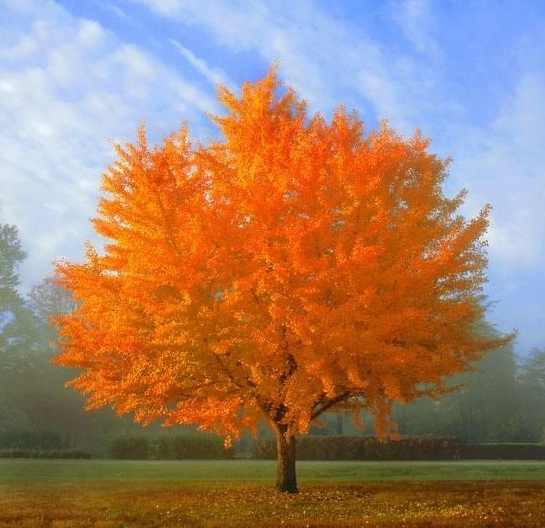
\includegraphics[width=\linewidth]{tree.jpg}
  \caption{Average return during the gradient ascent}
  \label{fig:sub3}
\end{subfigure}%
\begin{subfigure}{.5\textwidth}
  \centering
  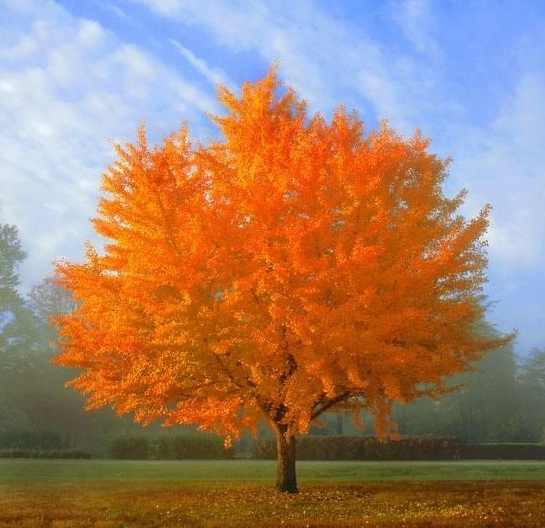
\includegraphics[width=\linewidth]{tree.jpg}
  \caption{Mean parameter during the gradient ascent}
  \label{fig:sub4}
\end{subfigure}%
\end{figure}



\end{document}
